%!TEX root = /Users/ego/Boulot/TKZ/tkz-graph/doc-fr/TKZdoc-gr-main.tex

% $Id$
\section{Vertex}
% The ( < name >) is a name for later reference and it is optional. You may also add the option name=< name > 
% to the < option > list; it has the same effect.
%<------------------------------------------------------------------------–> 
C'est bien évidemment la macro essentielle qui permet de placer des sommets. Les sommets peuvent être placés avec un système de coordonnées rectangulaires ou bien polaires ou encore relativement les uns par rapport aux autres. Quelques dispositions particulières sont également possibles.

\subsection{\tkzcname{Vertex}}
\begin{NewMacroBox}{Vertex}{\oarg{local options}\var{Name}}
Un sommet se caractérise par~:
\begin{itemize}
\item   sa référence,
\item   sa position,
\item   son label,
\item   et le style.
\end{itemize}

\medskip
Un argument non vide \IargName{Vertex}{Name} est obligatoire. Cet argument définit le nom de référence du  node. C'est celui que l'on doit utiliser dans toute création de sommet (\tkzcname{Vertex}) Il ne faut pas le confondre avec  le \tkzname{label} (étiquette) qui sera utilisé pour l'affichage.
On peut vouloir afficher $M_1$ alors que le nom lui sera $M1$.

\medskip
Des options sont utilisées pour définir les quatre premières caractéristiques. Les styles texte et graphique sont traités séparément.  

\medskip
\begin{tabular}{llc}
\midrule
Options   & Défaut  & Définition              \\
\midrule
\TOline{x}        {\{\}}{abscisse}  
\TOline{y}        {\{\}}{ordonnée}   
\TOline{a}        {\{\}}{angle}     
\TOline{d}        {\{\}}{distance}   
\TOline{Node}     {false}{utilisation d'une référence déjà définie}   
\TOline{position} {\{\}}{style qui permet un positionnement relatif }   
\TOline{dir} {\textbackslash EA}{direction pour un positionnement relatif }   
\midrule 
\TOline{empty}    {false}{booléen permettant de ne pas afficher le sommet}   
\midrule 
\TOline{NoLabel} {false}{booléen supprime le label}  
\TOline{LabelOut}{false}{booléen Label extérieur au node}  
\TOline{L}       {\{\}}{Le label}  
\TOline{Math}     {false}{booléen qui affiche le label en mode math} 
\TOline{Ldist}   {0cm  }{distance du label au node} 
\TOline{Lpos}    {0    }{position du label par rapport au node} 
\bottomrule
\end{tabular}

\medskip
\emph{Cette macro permet de définir un sommet qui a un nom \tkzname{name} et un label.\\
Si \tkzname{L}$=${} alors \tkzname{label} = \tkzname{Name} sinon \tkzname{label} = \tkzname{L}.}
\end{NewMacroBox}

\subsubsection{Utilisation de coordonnées cartésiennes} 
\tkzcname{Vertex[x=\meta{number},y=\meta{number}]\var{name}}.  Coordonnées cartésiennes $x$ et $y$.

\begin{tkzexample}[latex=7cm,small]
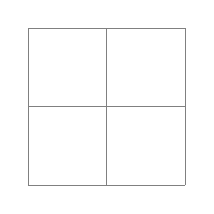
\begin{tikzpicture}
   \GraphInit[vstyle=Normal]
   \draw[help lines] (0,0) grid (2,2);
   \Vertex{A} % par défaut x = 0 et y = 0
   \Vertex[x=2 , y=0]{B} \Vertex[x=2 , y=2]{C}
\end{tikzpicture}
\end{tkzexample}

\subsubsection{Utilisation de coordonnées polaires} 

 \tkzcname{Vertex[a=\meta{number},d=\meta{number}]\var{vertex}} Les coordonnées polaires peuvent être aussi utilisées. J'ai utilisé une grille d'aide afin de constater le placement du sommet. 


\begin{tkzexample}[latex=7cm,small] 
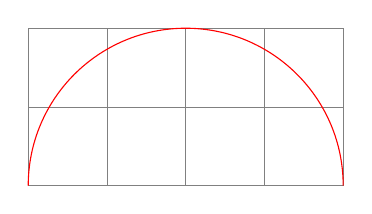
\begin{tikzpicture}
   \GraphInit[vstyle=Normal]
   \draw[help lines] (-2,0) grid (2,2);
   \draw[red] (2,0) arc (0:180: 2 cm);
   \Vertex{A}
   \Vertex[a=45 , d=2 cm]{B}
   \Vertex[a=135 , d=2 cm]{C}
\end{tikzpicture}
\end{tkzexample} 
 


 

\subsubsection{Option \tkzname{Node} : utilisation d'une position référencée} 
Cette option permet de placer un sommet sur un Node déjà défini ou bien
 un objet du type \og~coordinate~\fg.
   % pb taile du node pour M ??
\begin{tkzexample}[latex=7cm,small]
\begin{tikzpicture}
   \GraphInit[vstyle=Normal]
   \draw[help lines] (0,0) grid (2,2);
   \Vertex{A} \Vertex[x=2 , y=2]{B}
   %\tkzActivOff  nécessaire avec frenchb et babel
   \tkzActivOff 
   \coordinate (M) at ($ (A)!.5!(B) $){};
   \tkzActivOn
   \Vertex[Node]{M}
\end{tikzpicture}
\end{tkzexample}

\vfill
%<------------------------------------------------------------------------–>
%                             ShortCuts
%<------------------------------------------------------------------------–>

\newpage
\subsection{Raccourcis pour placement relatif}

Pour effectuer des placements relatifs, il est nécessaire de définir une distance unité entre deux sommets. La macro suivante permet de définir cette distance.

\begin{NewMacroBox}{SetGraphUnit}{\var{nombre}}
\emph{Cette macro permet de définir la distance entre deux sommets. La distance se réfère aux centres de ces sommets et le nombre est exprimé en \tkzname{cm}. Par défaut, l'unité est $1$ cm.}

utilisation :\tkzcname{SetGraphUnit\{2\}} 
\end{NewMacroBox}

\begin{NewMacroBox}{ShortCut}{\oarg{local options}\varp{vertex A}\var{vertex B}}
Ces raccourcis permettent de créer un \tkzname{vertex B}  relativement à un 
\tkzname{vertex A}. La distance entre les deux sommets est déterminé par  la valeur de \tkzname{unit} et par les unités de \TIKZ. Horizontalement et verticalement la distance est définie par \tkzname{unit}$\times$\tkzname{x} et 
\tkzname{unit}$\times$\tkzname{y}. La valeur de \tkzname{unit} peut être redéfinie par la macro  \tkzcname{SetGraphUnit} ou bien avec l'option \tkzname{unit}. Avec l'option la définition est locale; avec la macro, la définition est globale mais elle peut être locale si elle est intervient dans un goupe \TEX ou un environnement \tkzname{scope}.
Les raccourcis sont :

\medskip
\begin{tabular}{lll}
\hline
Raccourcis   &   & Définition              \\
\midrule
\TMline{EA}    {}  {à l'est }        
\TMline{WE}    {}  {à l'ouest}         
\TMline{NO}    {}  {au nord}        
\TMline{SO}    {}  {au sud}        
\TMline{NOEA}  {}  {au nord-est soit "nord" puis "est"}  
\TMline{NOWE}  {}  {au nord-ouest soit "nord" puis "ouest" }   
\TMline{SOEA}  {}  {au sud-est soit "sud" puis "est"}  
\TMline{SOWE}  {}  {au sud-ouest soit "sud" puis "ouest"}   
\bottomrule
\end{tabular}

\medskip
\emph{\tkzcname{NOEA} est un raccourci pour \tkzcname{NO}\tkzcname{EA}. par défaut, la distance entre les sommets avec ce raccourci est $\sqrt{2}\times$ \tkzname{unit}=$\sqrt{2}$. Les options sont celles de la macro \tkzcname{Vertex}. }
\end{NewMacroBox} 

Nous allons d'abord modifier la distance entre deux noeuds d'une façon générale avec \tkzcname{SetGraphUnit\{2\}} sinon par défaut \tkzname{unit =1}. 

\subsubsection{Utilisation des raccourcis avec les valeurs par défaut} 
\begin{tkzexample}[latex=7cm,small]
\begin{tikzpicture}
   \draw[help lines] (-1,-1) grid (1,1);
   \GraphInit[vstyle=Normal]
   \Vertex{A}
   \EA(A){B}   \WE(A){C}   \NO(A){D}   \SO(A){E}
   \NOEA(A){F} \NOWE(A){G} \SOEA(A){H} \SOWE(A){I}
   \foreach \v in {B,C,D,E,F,G,H,I}{\Edge(A)(\v)};
\end{tikzpicture}
\end{tkzexample} 


\subsubsection{Modification de l'unité avec  \tkzcname{SetGraphUnit }} 
\begin{tkzexample}[latex=7cm,small]
\begin{tikzpicture}
   \draw[help lines] (-2,-2) grid (2,2);      
   \SetGraphUnit{2}
   \GraphInit[vstyle=Normal]
   \Vertex{A}
   \EA(A){B}   \WE(A){C}   \NO(A){D}   \SO(A){E}
   \NOEA(A){F} \NOWE(A){G} \SOEA(A){H} \SOWE(A){I}
   \foreach \v in {B,C,D,E,F,G,H,I}{\Edge(A)(\v)};
\end{tikzpicture}
\end{tkzexample} 

\subsubsection{Modification des unités de \TIKZ\ : \tkzname{x=2 cm,y=1 cm} } 
\begin{tkzexample}[latex=7cm,small]
\begin{tikzpicture}[x=2 cm,y=1 cm]
   \draw[help lines] (-1,-1) grid (1,1);      
   \GraphInit[vstyle=Normal]
   \Vertex{A}
   \EA(A){B}   \WE(A){C}   \NO(A){D}   \SO(A){E}
   \NOEA(A){F} \NOWE(A){G} \SOEA(A){H} \SOWE(A){I}
   \foreach \v in {B,C,D,E,F,G,H,I}{\Edge(A)(\v)};
\end{tikzpicture}
\end{tkzexample} 


\subsubsection{Exemple classique} 
\begin{tkzexample}[latex=7cm,small]
\begin{tikzpicture}
   \draw[help lines] (-2,-2) grid (4,2);     
  \SetGraphUnit{2}
  \coordinate (O) at (0,0);
  \NOEA(O){A} \NOWE(O){B} \SOEA(O){D} 
  \SOWE(O){C} \NOEA(D){E}
  \Edges(B,C,D,A,E,D,B,A,C)
\end{tikzpicture}
\end{tkzexample}

\subsubsection{Autre exemple classique}   
\begin{tkzexample}[latex=7cm,small]
\begin{tikzpicture}
   \draw[help lines] (0,-2) grid (4,2);
   \SetGraphUnit{2}
   \GraphInit[vstyle=Normal]
   \Vertex{A}
   \EA(A){B} \NO(B){C} \SO(B){D} \EA(B){E}
   \Edges(A,B,C,A,D,E,C)
\end{tikzpicture}
\end{tkzexample}


\subsubsection{Modication locale de \tkzname{unit} avec l'option}
Le plus simple  :
\begin{tkzexample}[latex=7cm,small]
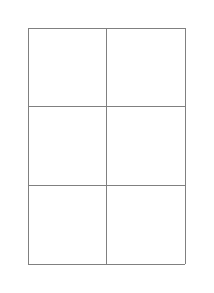
\begin{tikzpicture}
  \draw[help lines] (0,0) grid (2,3);
  \SetGraphUnit{2}
  \Vertex{A}  \EA(A){B} 
  \NO[unit=3](B){C}
  \NO(A){D}
\end{tikzpicture}
\end{tkzexample} 


\subsubsection{Modication locale de \tkzname{unit} avec l'environnement \tkzname{scope}}
\begin{tkzexample}[latex=7cm,small]   
 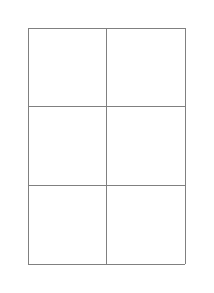
\begin{tikzpicture}
  \draw[help lines] (0,0) grid (2,3);
  \SetGraphUnit{2}
  \Vertex{A}  \EA(A){B} 
 \begin{scope}
    \SetGraphUnit{3} \NO(B){C}
 \end{scope}
 \NO(A){D}
\end{tikzpicture}
\end{tkzexample}     

\subsubsection{Modication locale de \tkzname{unit} avec un groupe \TEX}
\begin{tkzexample}[latex=7cm,small]   
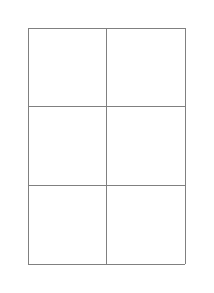
\begin{tikzpicture}
  \draw[help lines] (0,0) grid (2,3);
  \SetGraphUnit{2}
  \Vertex{A}  \EA(A){B} 
 {\SetGraphUnit{3} \NO(B){C}}
 \NO(A){D}
\end{tikzpicture}
\end{tkzexample} 

\endinput

